\chapter{Dataset}

I dataset utilizzati in questo lavoro sono due: \emph{EPIC-KITCHENS} \cite{Damen2021PAMI}, utilizzato nativamente da AMEGO per la costruzione del benchmark discusso in precedenza (AMB), ed \emph{ENIGMA-51} \cite{ragusa2023enigma51}, oggetto principale del lavoro di tesi e rifinito nel formato AMEGO per valutare il metodo su un contesto differente.

\section{EPIC-KITCHENS}
EPIC-KITCHENS è un dataset egocentrico raccolto in contesti domestici di cucina. Contiene registrazioni video di attività quotidiane svolte da singoli individui in cucina, con annotazioni di azioni e oggetti coinvolti. 

\subsection*{Collezione dei dati}
Il dataset è stato registrato da 32 partecipanti, ciascuno dei quali ha documentato tutte le visite in cucina. Le registrazioni iniziavano immediatamente prima dell'ingresso in cucina e terminavano appena prima dell'uscita. I partecipanti erano soli in cucina durante le registrazioni, in modo da catturare esclusivamente attività di una singola persona.  

La cattura dei dati è stata effettuata mediante una GoPro montata in testa, con un supporto regolabile per adattarsi all'altezza dei diversi soggetti e all'ambiente.  

\begin{figure}[ht]
    \centering
    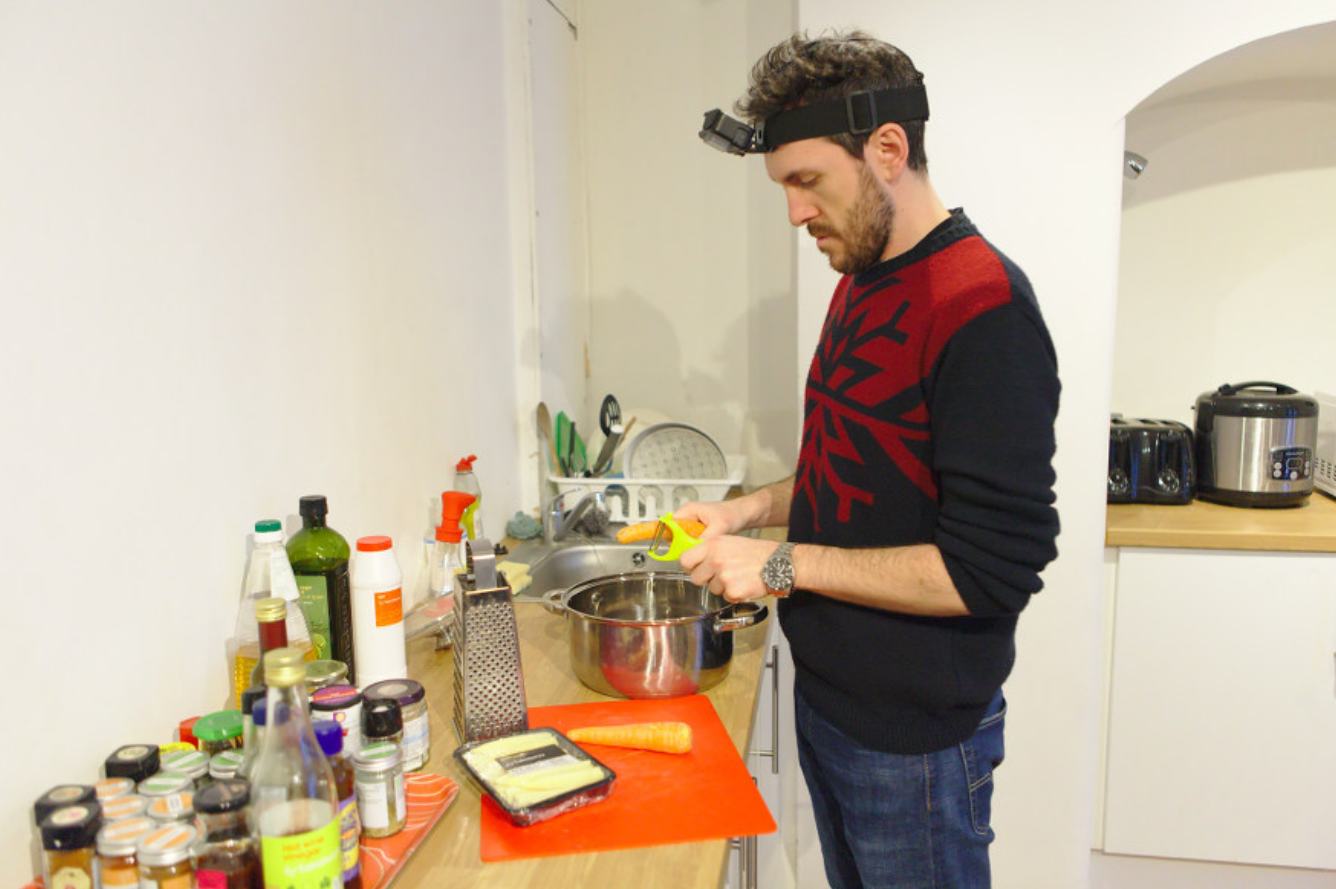
\includegraphics[width=0.6\textwidth]{Images/goproepic.png}
    \caption{Modalità di ripresa con GoPro montata in testa}
\end{figure}

Le riprese sono in risoluzione Full HD di 1920x1080 a 59.94 fps. Alcune registrazioni avevano risoluzioni o frame rate differenti: 1\% a 1280x720, 0.5\% a 1920x1440, 1\% a 30 fps, 1\% a 48 fps e 0.2\% a 90 fps.

In media, le registrazioni hanno una durata di 1.7 ore, con un massimo di 4.6 ore per soggetto.

\subsection*{Annotazioni}
La pipeline di annotazione ha avuto inizio con una prima fase di narrazione da parte dei partecipanti stessi, seguita da un processo di crowdsourcing su Amazon Mechanical Turk (AMT) \cite{mturk} per la rifinitura e la validazione dei dati \cite{Damen2021PAMI}. Le annotazioni raccolte si dividono principalmente in tre tipologie: narrazioni video, segmenti di azione e bounding box degli oggetti.

\subsubsection* {Narrazioni Video}
Come primo passo, è stato chiesto ai partecipanti di guardare i propri video dopo aver completato tutte le registrazioni e di narrare a voce le azioni che avevano compiuto \cite{Damen2021PAMI}. Le narrazioni sono state raccolte in 5 lingue diverse (inglese, italiano, spagnolo, greco e cinese), a seconda della lingua madre del partecipante \cite{Damen2021PAMI}.

Successivamente, queste registrazioni audio sono state trascritte manualmente tramite AMT, poiché i sistemi di speech-to-text automatici \cite{google_speech,ibm_watson,cmu_sphinx} si sono rivelati inefficaci a causa del lessico specifico e delle frasi incomplete \cite{Damen2021PAMI}. I timestamp di ogni narrazione sono stati ottenuti allineando l'audio al video tramite lo strumento di sottotitolaggio automatico di YouTube. Questo processo ha portato alla raccolta di 39,596 narrazioni di azioni.

\subsubsection* {Segmenti di Azione}
Le narrazioni hanno fornito una prima localizzazione temporale approssimativa delle azioni \cite{Damen2021PAMI}. Per ottenere una segmentazione precisa, per ogni frase narrata, i tempi esatti di inizio e fine dell'azione corrispondente sono stati annotati tramite un ulteriore task su AMT \cite{Damen2021PAMI}. In questo modo, sono stati etichettati 39,564 segmenti di azione, con una durata media di 3.7 secondi \cite{Damen2021PAMI}.

\begin{figure}[ht]
    \centering
    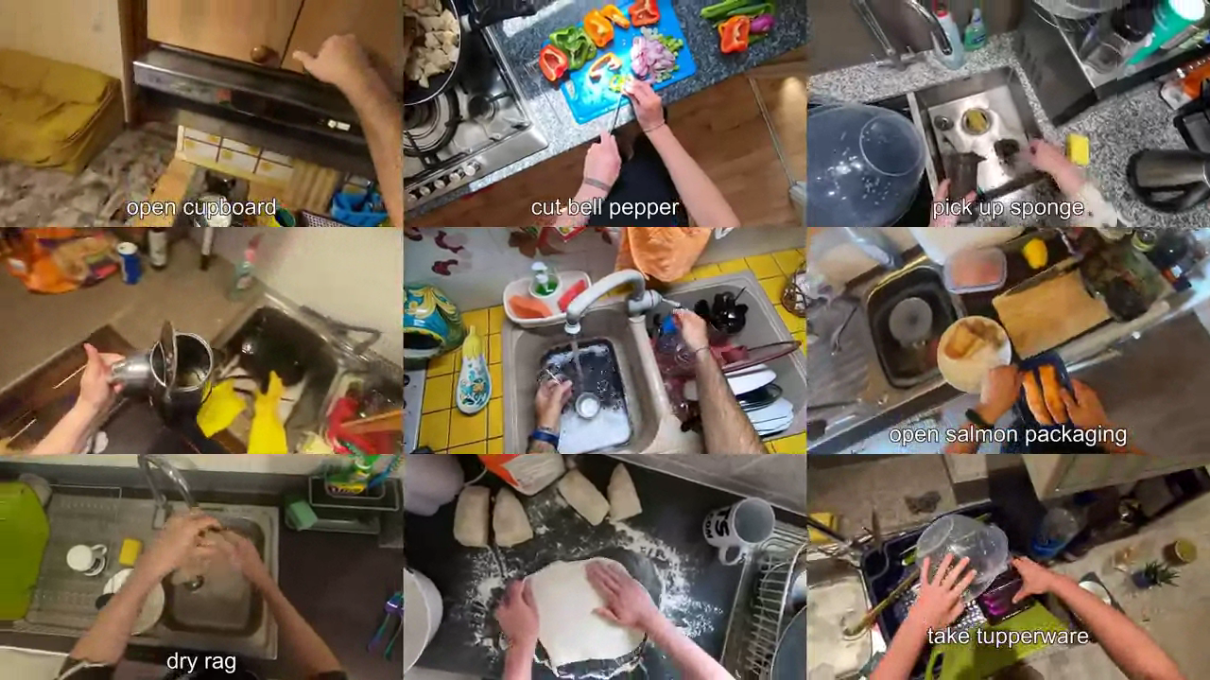
\includegraphics[width=0.8\linewidth]{Images/epic_ex.png}
    \caption{Esempi di azioni annotate in EPIC-KITCHENS}
    \label{fig:amb_stats2}
\end{figure}

\subsubsection* {Bounding Box degli Oggetti Attivi}
I sostantivi presenti nelle narrazioni sono stati usati come riferimento per annotare gli oggetti con cui il partecipante interagiva (definiti "oggetti attivi") \cite{Damen2021PAMI}. Per ogni sostantivo menzionato in un segmento di azione, sono stati estratti i fotogrammi all'interno e immediatamente prima/dopo il segmento temporale ($[t_s - 2s, t_e + 2s]$) \cite{Damen2021PAMI}. Su questi frame, i lavoratori di AMT sono stati incaricati di disegnare i bounding box attorno agli oggetti specificati \cite{Damen2021PAMI}. In totale, sono stati raccolti 454,255 bounding box \cite{Damen2021PAMI}.

\begin{figure}[ht]
    \centering
    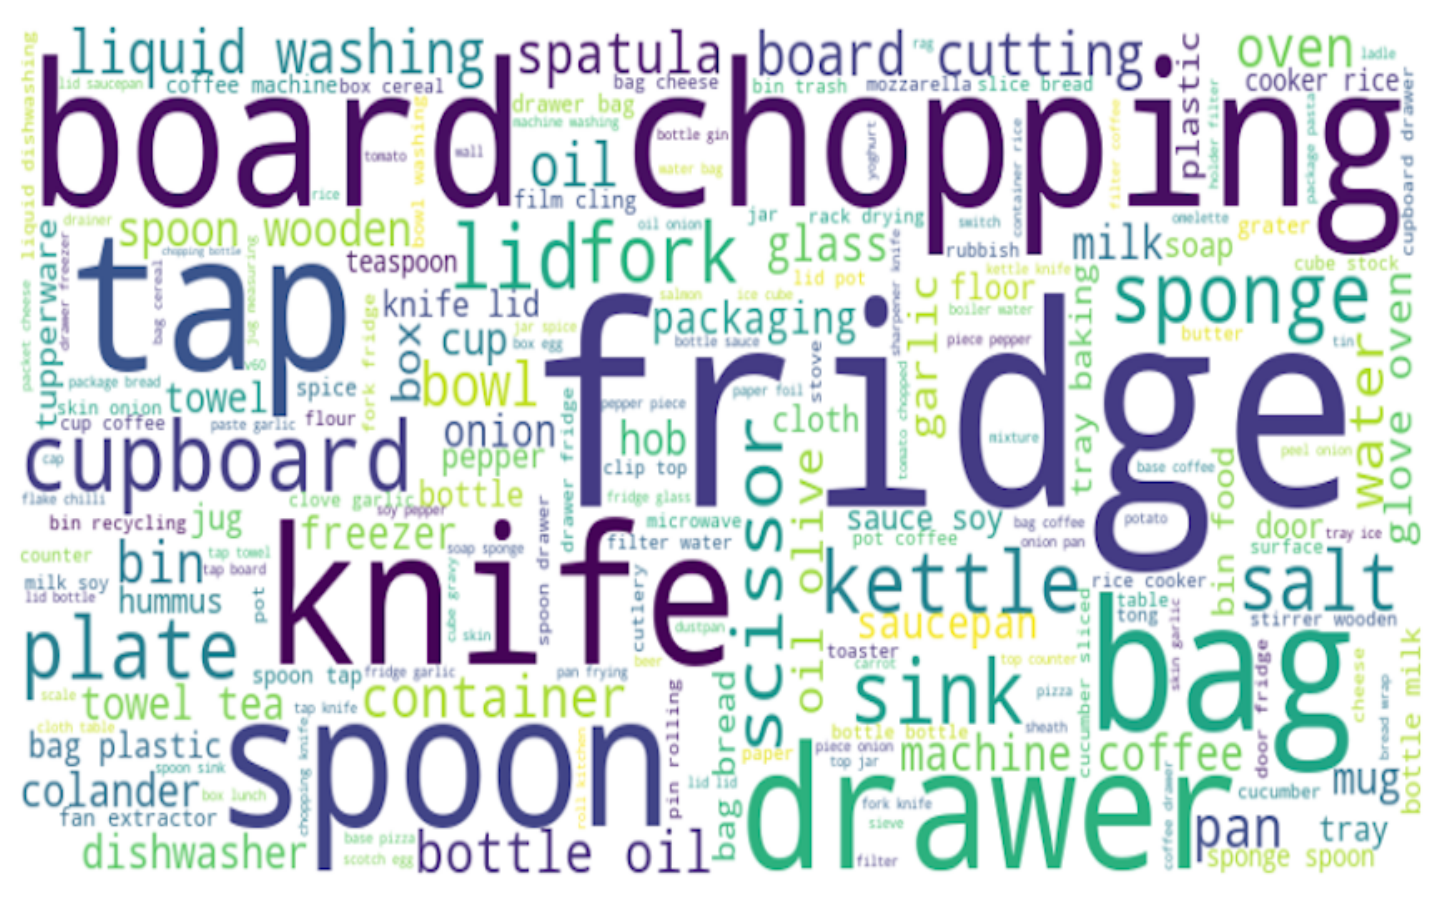
\includegraphics[width=0.6\linewidth]{Images/epic_cloud.png}
    \caption{Wordcloud degli oggetti interrogati di frequente}
    \label{fig:amb_stats1}
\end{figure}

\subsection*{AMB}
Partendo da queste annotazioni, è stato possibile creare la ground truth per il benchmark \emph{Active Memories Benchmark} (AMB). L'AMB è un benchmark di tipo \emph{visual-only QA}, perciò uno dei principali problemi da affrontare è la selezione di una rappresentazione visiva degli oggetti per costruire le \emph{visual query} (VQ). Per gestire l'occlusione tipica dei video egocentrici, causata dalle mani del soggetto o da altri oggetti, per ogni oggetto sono stati selezionati fino a tre \emph{image patch} differenti, sufficientemente distanti temporalmente (almeno 0.5s tra una patch e l'altra) per mostrare pose differenti. Inoltre, sono state scelte patch con minima sovrapposizione spaziale con i bounding box di altri oggetti o mani attivi nello stesso frame.

Analogamente, per le location sono stati estratti i frame con minima sovrapposizione spaziale con gli oggetti attivi, in modo che la location fosse visibile senza la presenza di molti oggetti in movimento. Inoltre si è garantita una distanza minima temporale di 1s tra le immagini selezionate.  

Sono stati selezionati casualmente 100 video di EPIC-KITCHENS, dai quali sono state generate circa 20.5K queries in maniera semi-automatica. Ogni domanda è composta da cinque possibili opzioni. In particolare, le possibili risposte vengono selezionate in maniera differente a seconda del tipo di domanda. Nel paper originale sono fornite linee guida generiche per i vari template, ad esempio:

\begin{figure}[ht]
    \centering
    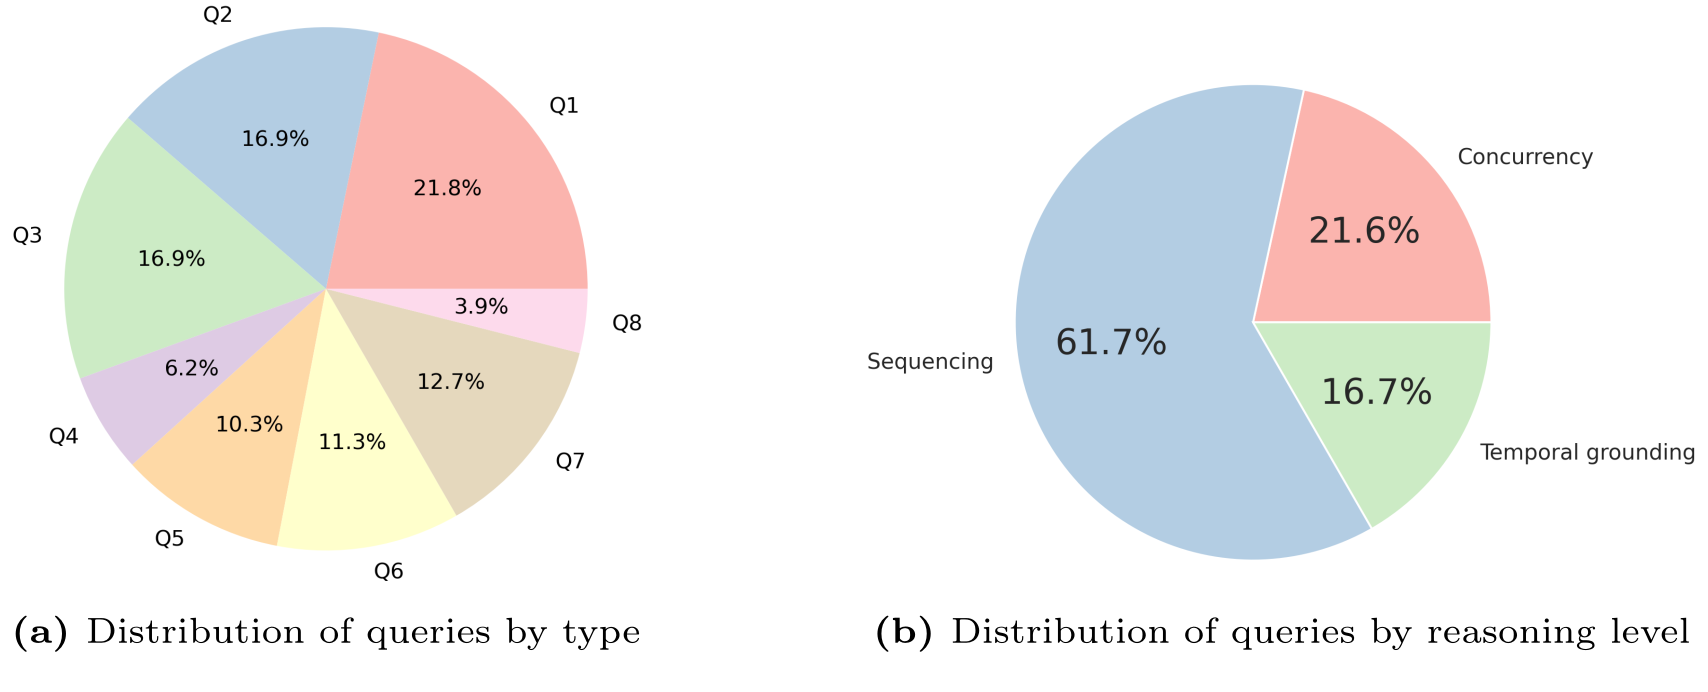
\includegraphics[width=0.7\linewidth]{Images/amb_stats.png}
    \caption{Distribuzioni dei tipi di query presenti in AMB}
    \label{fig:amb_stats0}
\end{figure}

\begin{itemize}
    \item \textbf{Q6}: le opzioni includono le location visitate immediatamente dopo che il soggetto ha interagito con un oggetto specifico;
    \item \textbf{Q3-Q4}: le opzioni possono includere oggetti utilizzati con la mano opposta;
    \item \textbf{Q2-Q3}: il tempo della query $t$ è fissato in modo tale che l'oggetto [VQ] non sia ancora stato utilizzato, richiedendo prima di individuare l'interazione con [VQ] e successivamente quelle precedenti o successive.
\end{itemize}

\section{ENIGMA-51}
ENIGMA-51 è un dataset egocentrico acquisito in uno scenario industriale, in cui 19 soggetti hanno seguito istruzioni per completare operazioni di riparazione di schede elettroniche utilizzando strumenti industriali (ad esempio cacciaviti elettrici) ed apparecchiature di laboratorio (ad esempio oscilloscopi).  

\begin{figure}[ht]
    \centering
    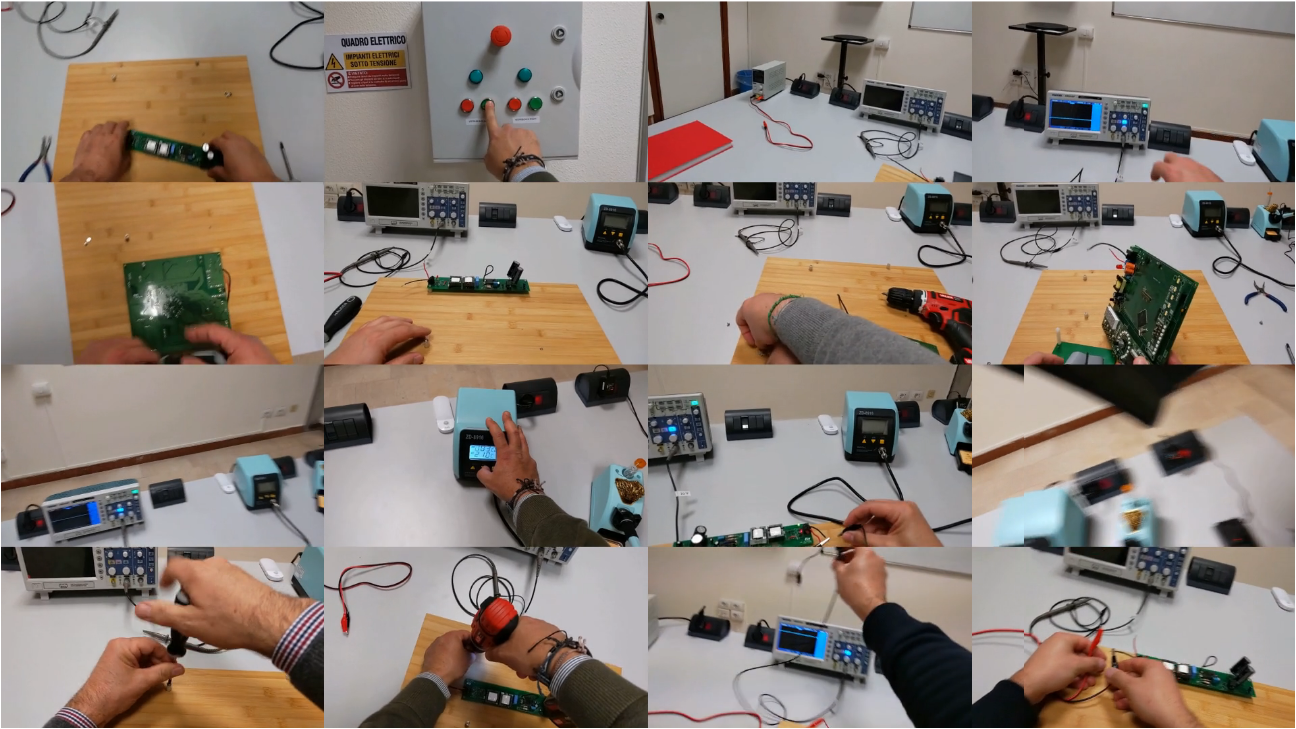
\includegraphics[width=0.8\linewidth]{Images/enigma_ex.png}
    \caption{Frame presenti nel dataset ENIGMA-51}
\end{figure}

\subsection*{Collezione dei dati}
Le sequenze sono state acquisite in uno scenario controllato che riproduce fedelmente un ambiente industriale. I partecipanti hanno indossato un visore \emph{Microsoft HoloLens 2}.

Le registrazioni sono caratterizzate da una risoluzione di $2272 \times 1278$ pixel e da un framerate di 30 fps. Ogni sequenza ha una durata media di circa 26 minuti, per un totale complessivo di 22 ore di materiale acquisito.  

Durante le riprese, i partecipanti hanno seguito istruzioni dettagliate per completare due procedure di riparazione, una a bassa e una ad alta tensione. Le indicazioni venivano fornite direttamente attraverso l'HoloLens 2 tramite un'applicazione dedicata, che combinava audio, immagini e contenuti di realtà aumentata per guidare l'utente passo dopo passo.

\subsection*{Annotazioni}
Le annotazioni coprono diversi livelli di dettaglio, dagli aspetti temporali alle interazioni mano-oggetto.

In tutti i 51 video sono stati individuati i \emph{key frame} di interazione con oggetti. Ciascuno viene fornito di un timestamp e da un verbo che descrive l'azione in corso.  

La tassonomia dei verbi comprende quattro azioni fondamentali:  
\begin{itemize}
    \item \emph{first-contact} (primo contatto)  
    \item \emph{de-contact} (fine del contatto)  
    \item \emph{take} (prendere)  
    \item \emph{release} (rilasciare)  
\end{itemize}

Nel complesso, sono state annotate \textbf{14.036 interazioni}.

\begin{figure}[ht]
    \centering
    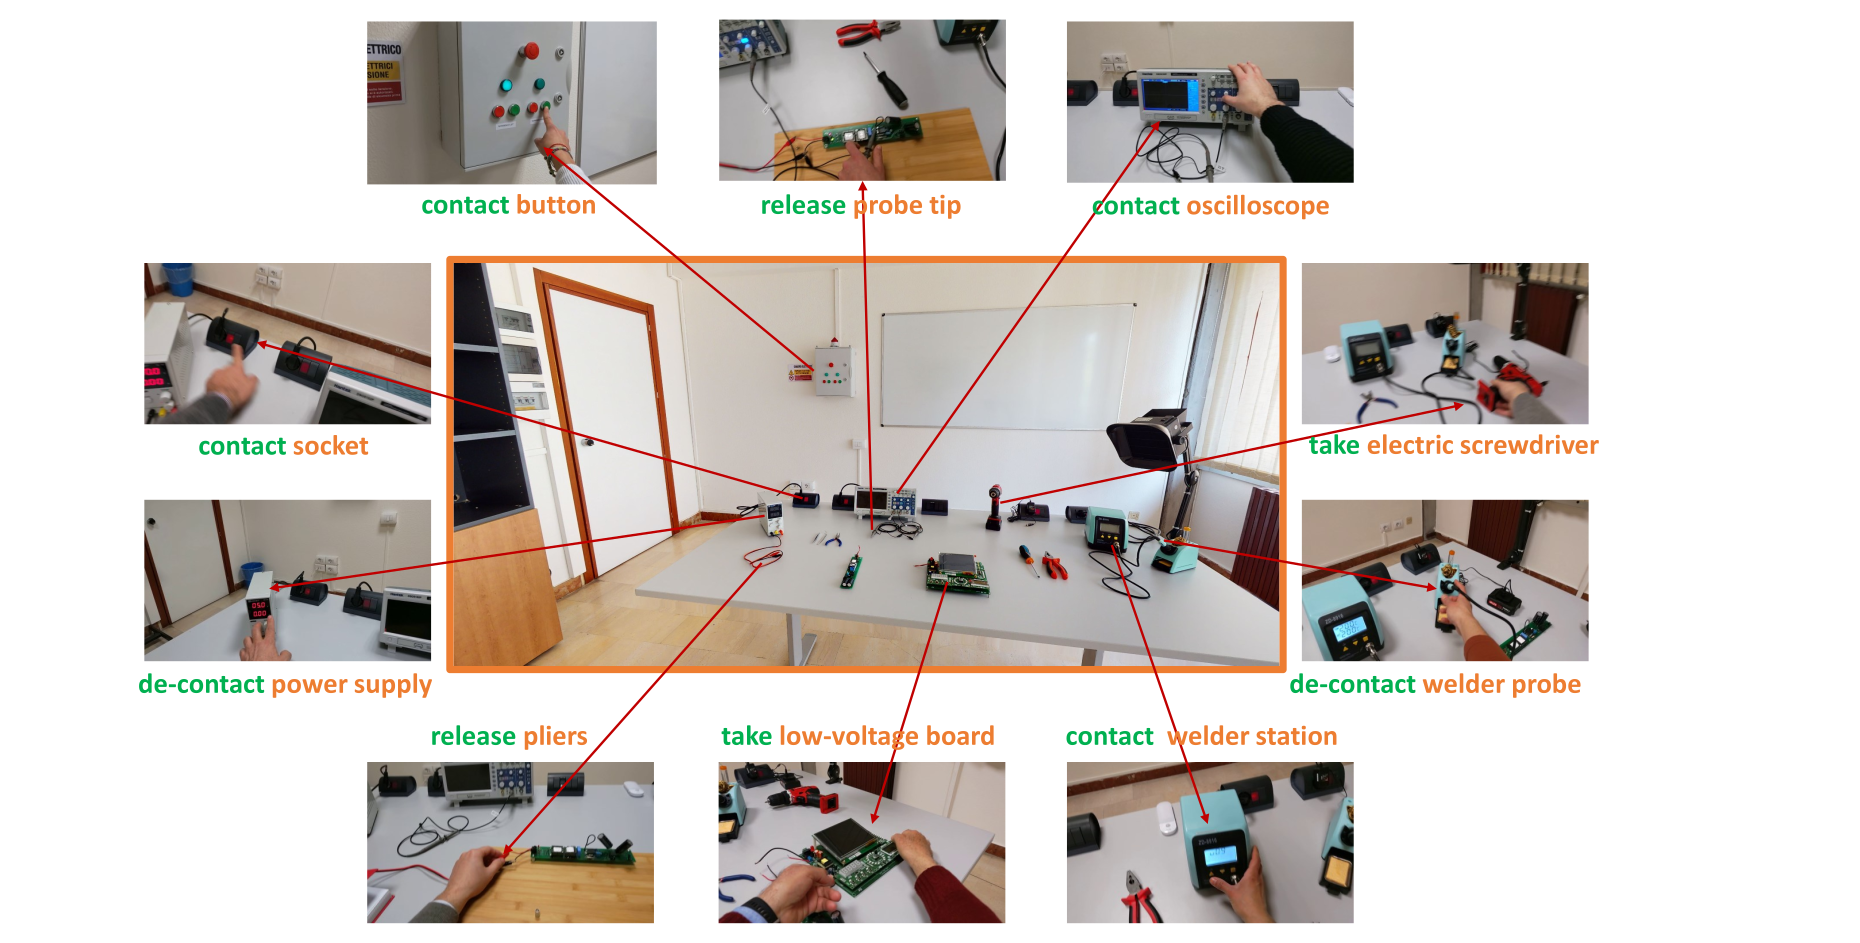
\includegraphics[width=1\linewidth]{Images/enigma_verbs.png}
    \caption{Esempi di azioni annotate in ENIGMA-51}
\end{figure}

Sono state definite 25 classi di oggetti, comprendenti sia oggetti fissi (ad esempio un pannello elettrico) sia strumenti mobili (come un cacciavite).  
Ogni oggetto è rappresentato attraverso una tupla che descrive la classe, le coordinate del rettangolo di delimitazione (\emph{bounding box}) e lo stato, che specifica se l'oggetto è attivo o passivo nell'interazione.  
Complessivamente, sono stati annotati \textbf{275.135 oggetti}.  

Sono stati etichettati i \emph{bounding box} delle mani.  
Per ciascuna mano è stato corretto manualmente il lato (destra o sinistra) e indicata l'associazione con l'oggetto attivo in interazione.  
In totale, le mani annotate ammontano a \textbf{56.473}.

Insieme alle varie annotazioni, il dataset fornisce ulteriori risorse utili per lo studio delle interazioni in contesti industriali.  
Sono inclusi i \textbf{modelli 3D} dell'ambiente e degli oggetti, così come due \textbf{procedure} composte da istruzioni che guidano l'utente nelle interazioni con gli oggetti stessi.

\subsection*{Active Memories Benchmark (AMB)}

La costruzione del benchmark ha usato metodologie analoghe a quelle riportate nel paper originale di AMEGO. I dettagli sono descritti nel Capitolo~\ref{cap:Esperimenti}.  

Di seguito sono riportate alcune statistiche rilevanti sul benchmark creato.

Nella figura \autoref{fig:enigma_chord} si evidenziano le associazioni tra le categorie di oggetti presenti tra le domande e la risposta corretta.

\begin{figure}[ht]
    \centering
    \begin{subfigure}[b]{0.32\textwidth}
        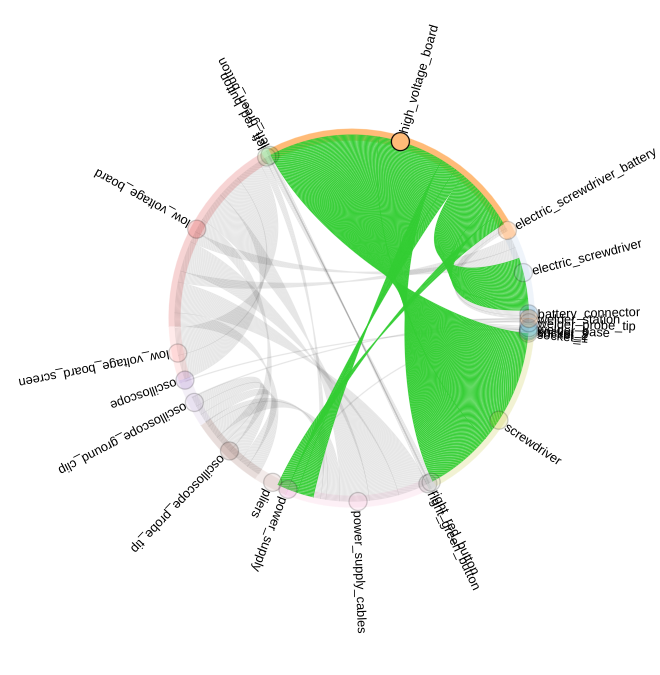
\includegraphics[width=\linewidth]{Images/enigma_amb_high_voltage.png}
        \caption{High Voltage (a)}
        \label{fig:high_voltage}
    \end{subfigure}
    \hfill
    \begin{subfigure}[b]{0.32\textwidth}
        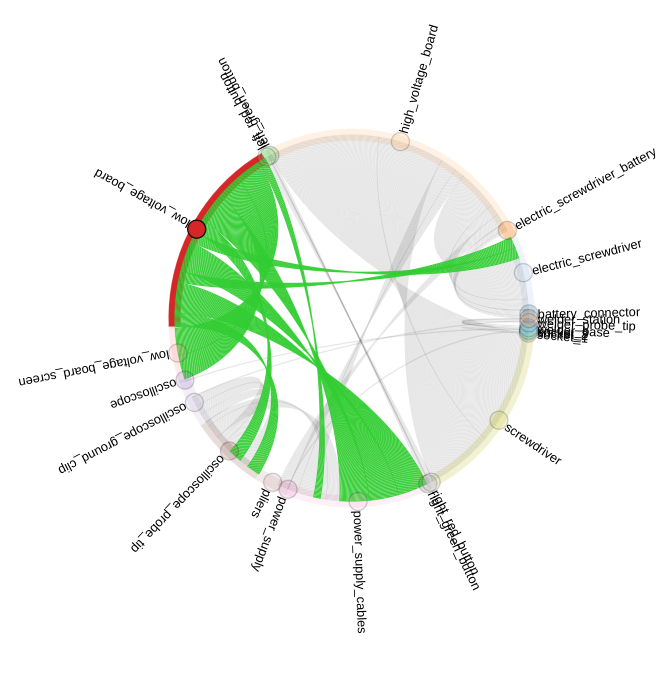
\includegraphics[width=\linewidth]{Images/enigma_amb_low_voltage.png}
        \caption{Low Voltage (b)}
        \label{fig:low_voltage}
    \end{subfigure}
    \hfill
    \begin{subfigure}[b]{0.32\textwidth}
        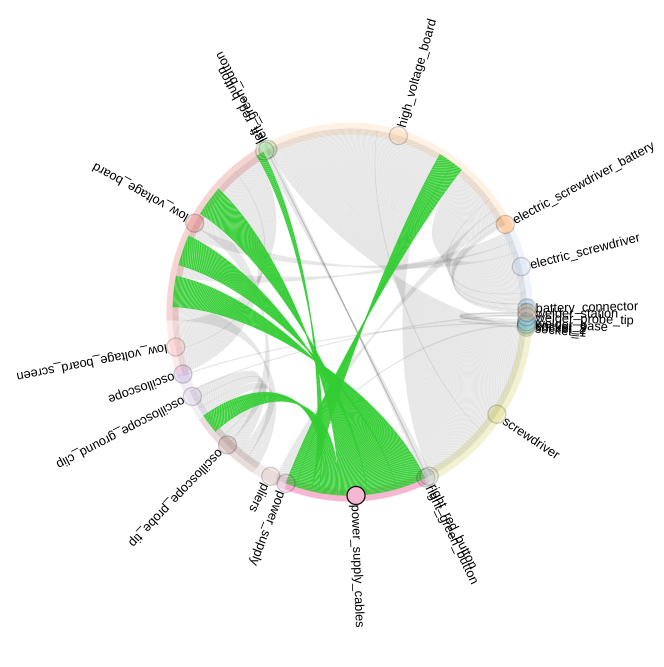
\includegraphics[width=\linewidth]{Images/enigma_amb_power_supply.png}
        \caption{Power Supply Cables (c)}
        \label{fig:power_supply}
    \end{subfigure}
    \caption{Chord diagrams che dimostrazione l'associazione tra categorie di oggetti nelle domande e la risposta corretta. Ogni subfigure corrisponde a un diverso tipo di procedura.}
    \label{fig:enigma_chord}
\end{figure}

Si notano a primo impatto gli elementi centrali del dataset. In particolare, le schede elettroniche ad alta e bassa tensione risultano essere le più frequenti e vengono comunemente utilizzate insieme a:
\emph{cacciavite}, \emph{sonda dell'oscilloscopio} e \emph{cavi di alimentazione}.
Per confermare queste osservazioni in maniera più quantitativa, è stata calcolata anche la matrice di correlazione tra le categorie (\autoref{fig:amb_corrmatrix}).

\begin{figure}[ht]
    \centering
    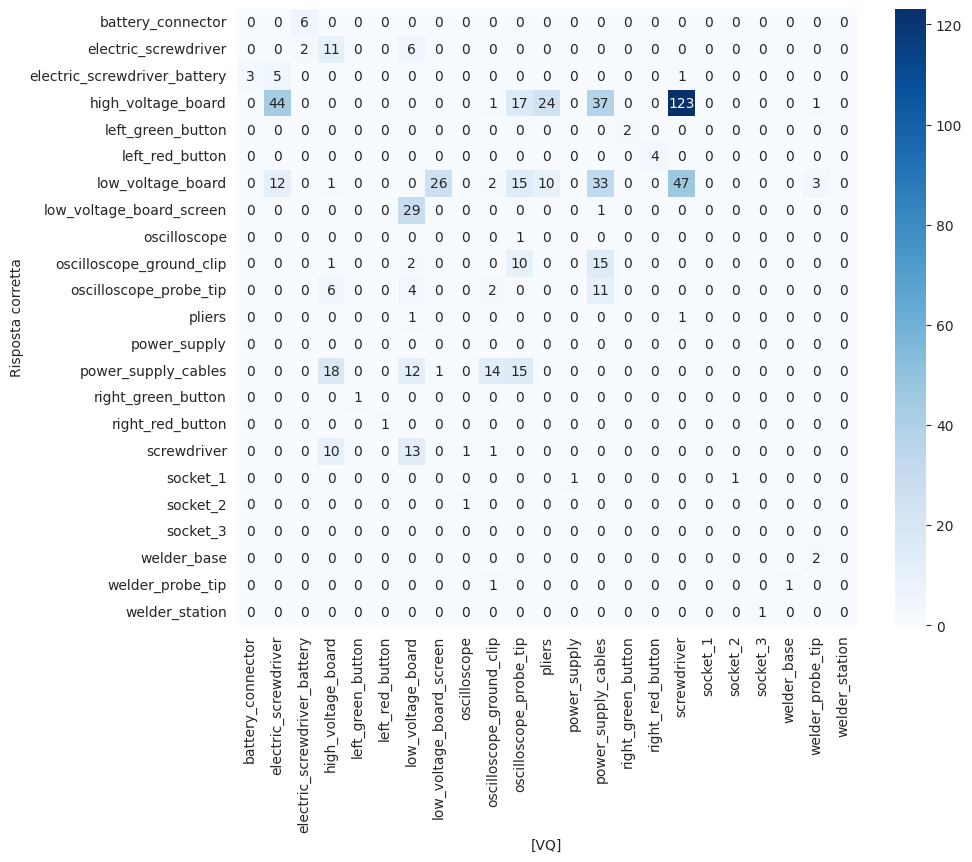
\includegraphics[width=1\linewidth]{Images/enigma_heat.png}
    \caption{Heatmap della distribuzione delle categorie degli oggetti nel benchmark AMB per ENIGMA-51.}
    \label{fig:amb_heatmap}
\end{figure}

Si conferma infatti che le interazioni più frequenti sono quelle con all'interno le schede elettroniche. queste interagiscono più di frequente con "screwdriver" "oscilloscope" "power supply" (lascia in eng e metti traduzione in ita tra parentesi).

\begin{figure}[ht]
    \centering
    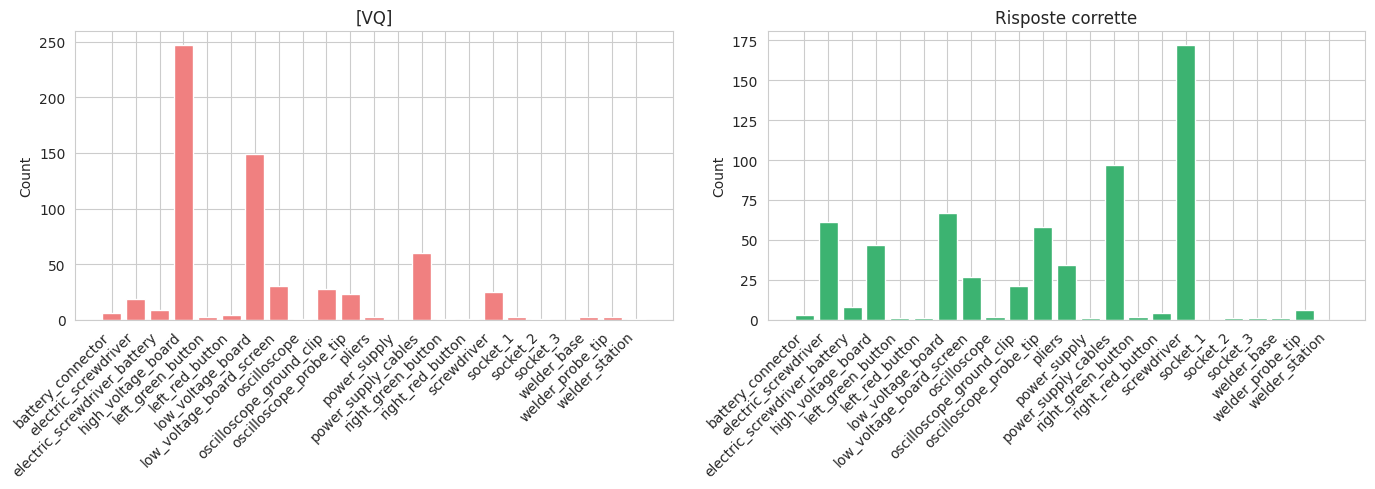
\includegraphics[width=1\linewidth]{Images/enigma_hist.png}
    \caption{Istogramma delle occorrenze delle categorie degli oggetti nel benchmark AMB per ENIGMA-51.}
    \label{fig:amb_corrmatrix}
\end{figure}